\chapter{Methodology}
\label{chap:methodology}



\section{System Design}
\label{sec:system-design}

Our neuro-symbolic planning system extends a re-implementation of the Generative Agents architecture \cite{parkGenerativeAgentsInteractive2023a} with modifications enabling controlled comparison between purely neural planning (baseline) and neuro-symbolic planning (our approach).

\subsection{System Architecture}
\label{subsec:system-architecture}

The implementation transforms the original monolithic Generative Agents codebase into a modular, service-oriented architecture:

\begin{enumerate}
    \item \textbf{Repository Layer}: Abstracts external dependencies (LLM APIs, file storage) behind interfaces. \texttt{LLMRepository} supports both OpenAI (production) and mock providers (testing). \texttt{EnvironmentRepository} abstracts world state persistence.

    \item \textbf{Service Layer}: Encapsulates cognitive capabilities in swappable interfaces:
          \begin{itemize}
              \item \texttt{PlanningService}: Daily planning and task decomposition
              \item \texttt{DialogueService}: Conversation generation
              \item \texttt{PerceptionService}: Environment observation and memory retrieval
              \item \texttt{ReflectionService}: Memory summarization
              \item \texttt{EnvironmentService}: Spatial navigation and object interaction
          \end{itemize}

    \item \textbf{Orchestration Layer}: The simulation loop consumes services through interfaces, configured via environment variables (\texttt{LLM\_PROVIDER}, \texttt{PLAN\_MODULE}) controlling which implementations run.
\end{enumerate}

\textbf{Key Design Principle}: The \texttt{PlanningService} abstraction enables side-by-side comparison of baseline (LLM-only hierarchical planning) and neuro-symbolic planning by ensuring both share identical environment state, memory retrieval, and LLM infrastructure. Only the planning logic differs, isolating the independent variable.

\begin{figure}[H]
    \centering
    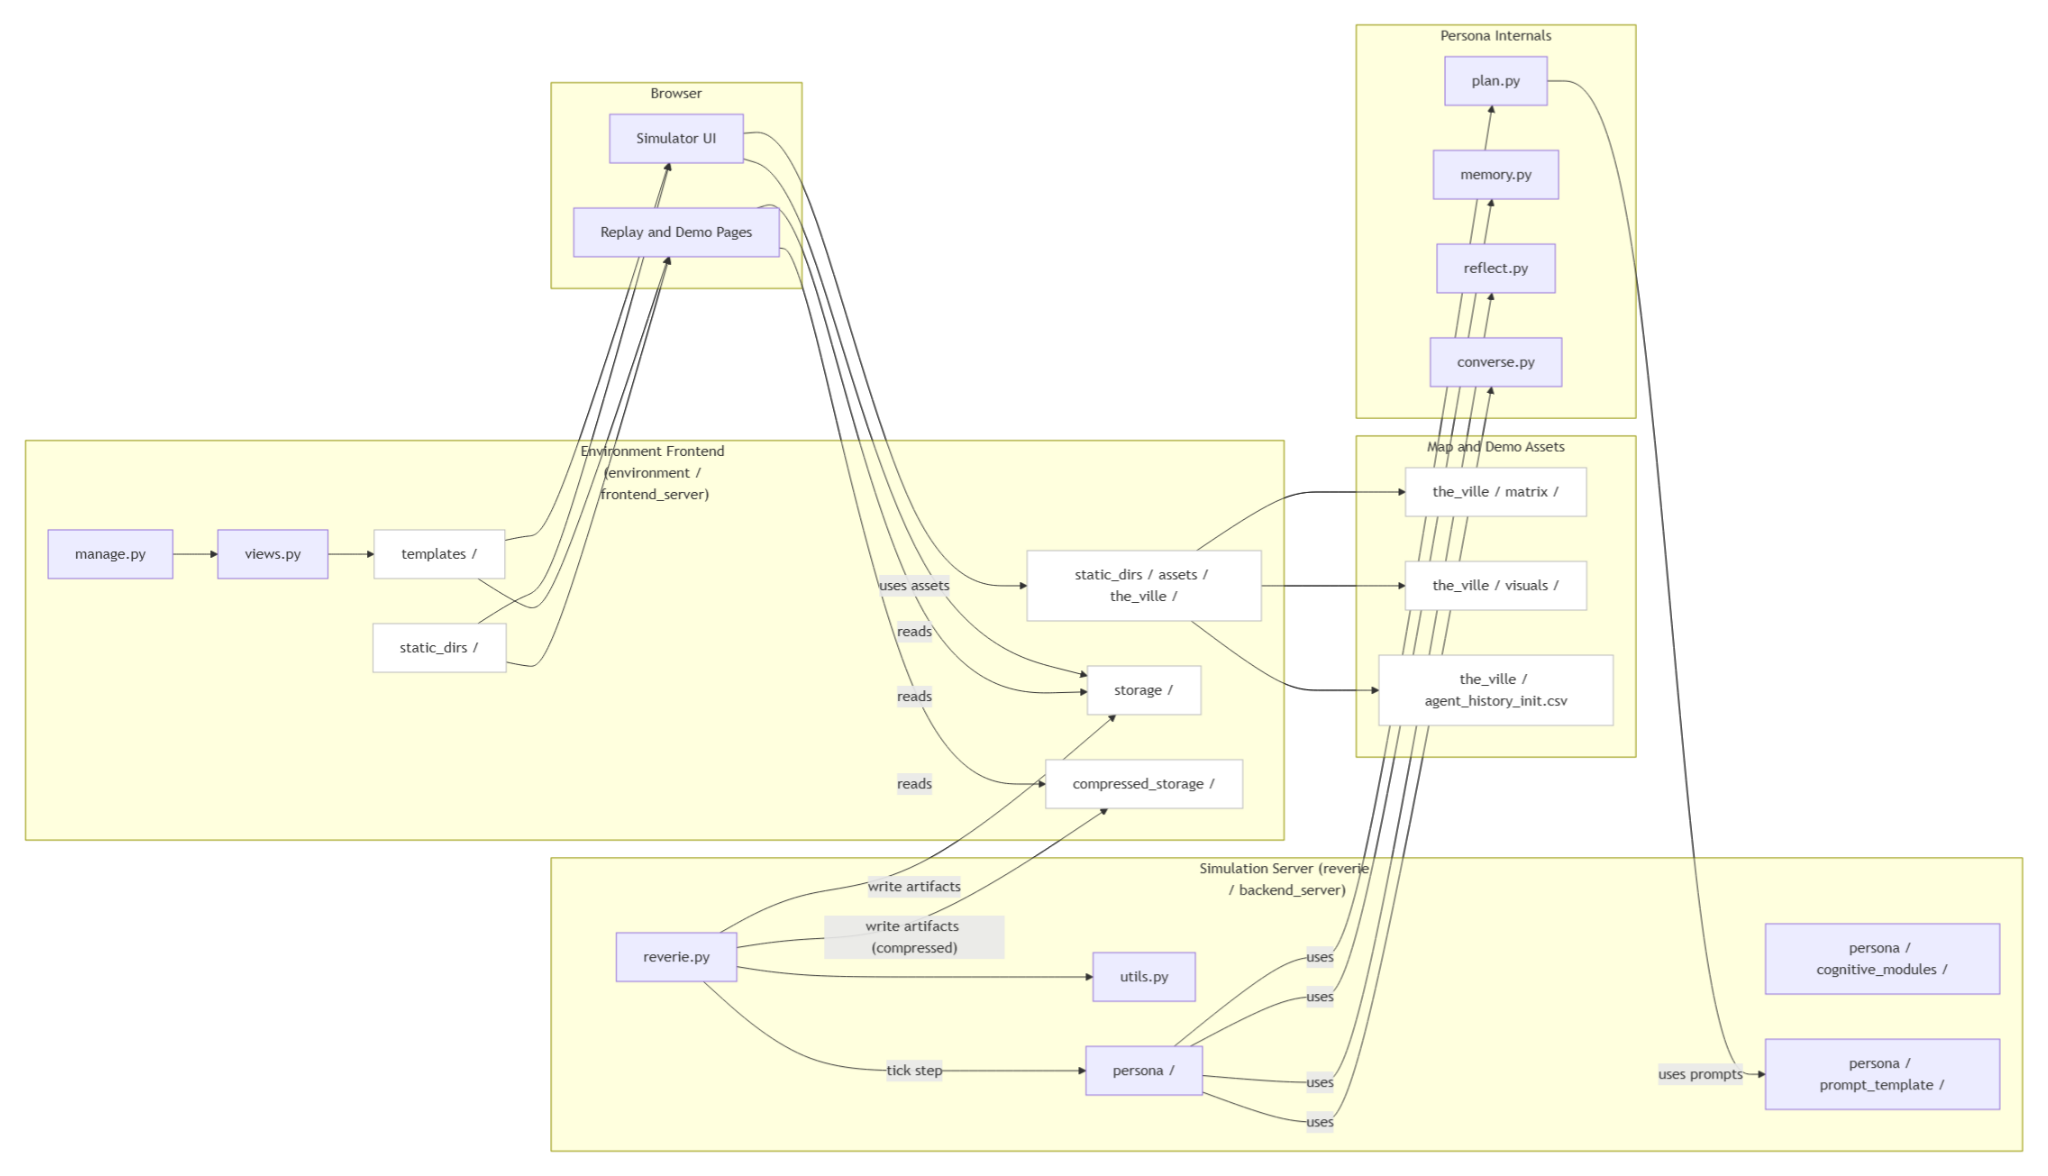
\includegraphics[width=\textwidth]{Pictures/Code Structure - before.png}
    \caption{Original monolithic architecture from the Generative Agents codebase \cite{parkGenerativeAgentsInteractive2023a}, showing tightly coupled components without clear separation of concerns.}
    \label{fig:code-structure-architecture-before}
\end{figure}

\begin{figure}[H]
    \centering
    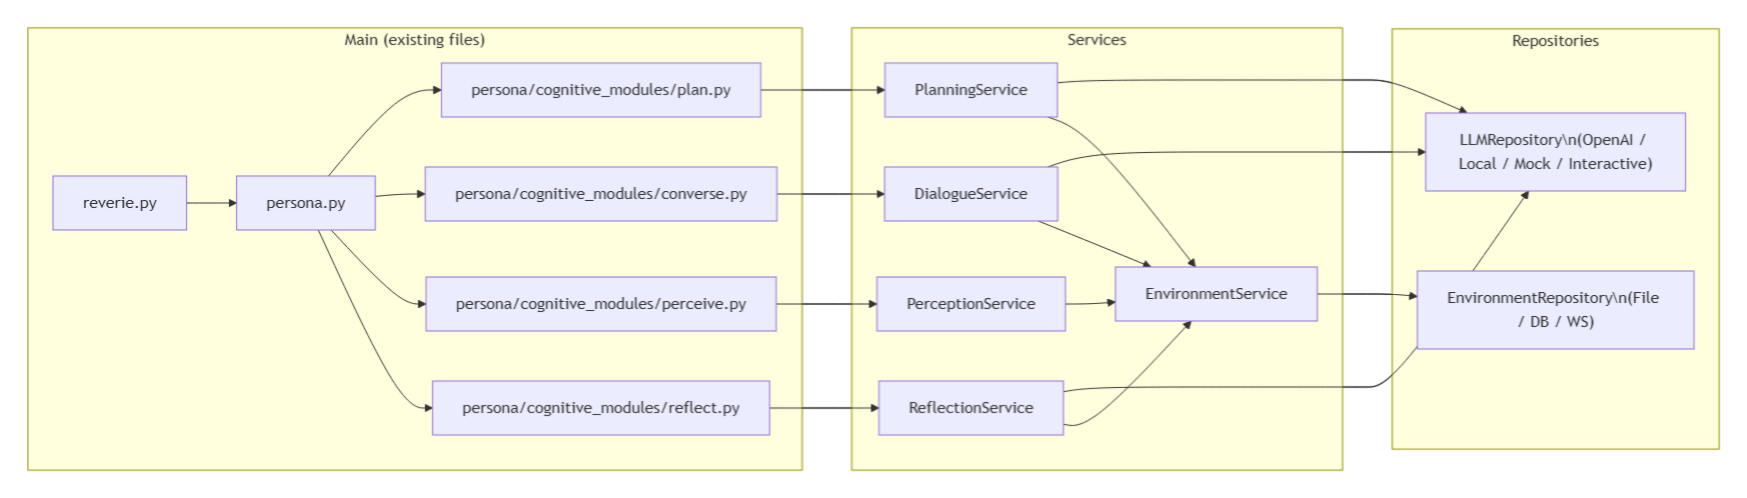
\includegraphics[width=\textwidth]{Pictures/Code Structure - after.png}
    \caption{Refactored service-oriented architecture with Repository, Service, and Orchestration layers. The \texttt{PlanningService} abstraction enables controlled comparison between baseline and neuro-symbolic planning implementations.}
    \label{fig:code-structure-architecture-after}
\end{figure}

\subsection{Prompt Templates}
All calls to the LLM are formalized using prompt templates, that specify the system prompt [Maybe add what is that], few-shot examples, templates for the actual prompt and expected output in a format using OpenAI structured output that allows us to put constraints on the model output. Also we get clear versioning of prompt templates.

\subsection{Model Used}
Most of the testing was done with the OpenAI model gpt-5-nano-2025-08-07, because of: 1. It's a cheap model which is important considering our expected token usage to generate one simulation was 1m+, 2. It's fast 3. It's a reasoning model with good benchmarks 4. It still allows for "intelligence" vs speed tradeoff by setting the reasoning token budget (reasoning effort between low, medium, and high)

[Should we write about other models as well?]

We were considering open source models like gpt-oss-120b

\subsection{Long-Term Planning}
\label{Long-term planning}
As part of improvements to the original architecture we modified the prompts responsible for the planning part, [of course also the code around].
\subsubsection{Movement}
The biggest change is the programmatic addition of movement actions. In the original paper the characters were moving as part of some determined actions so if an agent planned to eat breakfast for 20 minutes in a coffee shop that is 25 minutes from his current location, he would be walking to the café for 20 minutes and without even reaching the café he would start another activity. In our opinion this broke the believability of the original paper and we decided to automatically block time for the movement activity. That meant that the agent will always have the time to reach the destination before starting actions. But it also meant that when planning we need to estimate the time that the agent will spend on walking in each task as we get the action location only after decomposing the task into actions.


\subsubsection{Daily Planning}

In the original paper each of the big activities like "morning routine" was always generated as a multiple of one hour in terms of time. This was dictated by the poor reliability in producing structured output of the model that they used in the original study [GPT-3.5 Turbo]. With newer models and structured output we were able to ask the model to generate arbitrarily long tasks for a day. Another improvement is that we asked the model to generate task intent and location of interest in the task [So the area where the agent will most probably have to move during the execution of the task].
We used task intent as context for prompts that will operate on the task [replanning, task decomposition]. The locations of interest are used for estimating the travel time during the activity.

\subsubsection{Task Decomposition}
When an agent approaches a task that hasn't been decomposed yet, we trigger task decomposition into atomic actions. In the original implementation each action was a multiple of 5 minutes and that produced some unbelievable actions like washing hands for 5 minutes. In our implementation we let the model choose arbitrarily the amount of minutes. Then if we allow neuro-symbolic validation we enter the validation loop. Then with the final task decomposition we ask the model for the most appropriate place to do each of the actions. Then we programmatically generate movement actions if the agent needs to switch places in between actions. At the end we check if the total amount of time is above or below the expected amount of time for the task. Let's call it delta [The amount of time for task itself and amount of time expected for the movement]. If we need to fill up the time we add a "Checking phone" activity for |delta| minutes. If delta > 0 then we need to decrease time spent on actions. We do it by randomly decreasing the time of the activity by one minute [And we put more weight on the activities that take more time so a 20 minute activity will have ten times higher chance to be picked for decrease than a 2 minute activity] [make the examples more mathematically strict].



\subsection{Neuro-Symbolic Validation Pipeline}
\label{subsec:neuro-symbolic-pipeline}
We implemented the following neuro-symbolic validation pipeline in hopes of enhancing the coherence of actions generated as part of task decomposition. We do it after generating actions from the task, but before adding movements. [TODO add example] We do this by checking the validity of preconditions using the external symbolic validation tool VAL. To get feedback about the validity of the plan from VAL we need to generate 3 files: Domain.pddl, Problem.pddl and plan.pddl. Below we explain how we achieved this.

\subsubsection{Domain Generation}
Domain generation is the most difficult part of generation [Because it's the biggest mental load, maybe add statistics for this. I mean it's just that the domain needs the most attention and problems here will propagate to following steps of the pipeline] and we tested a couple of approaches to do it correctly. The steps below subjectively [We tested a lot and looked which generated more sensible results and which generated fewer validation errors] generated the best Domain. We started with trying to generate the whole PDDL file in one go based on the decomposed actions, but we got 2 problems: 1. the action conditions and effects tend to be chained without real logic to it. [add example, like teeth-brushed as precondition of shower]. So after many iterations we decided to split the domain generation into the following steps.

    [Also we use the structured JSON output to ensure proper naming and structure and we should write about it]

\paragraph{Natural Language Precondition and Effect Generation}
We ask the model for natural language conditions and effects of each action separately to prevent the chained condition-effect problem that we observed when generating the whole domain in one go. [add example]

\paragraph{Predicates Generation}
We gather all the natural language conditions and effects of each action and world description and ask the model to create a sensible predicate with focus on logical coherence. We do it in one go so we end up with a unified set of predicates. As the domain is unique for a specific agent and specific task decomposition we ask the model to generate zero-arity predicates as we saw that decreases the amount of hallucination and malformed output from LLMs in the next stages of the pipeline [Add example]


\paragraph{PDDL Action Schema Generation}
Now for each action we generate an action schema from the predicate catalog and natural language conditions and effects. We do it separately for each action to not encourage condition and effect chaining. After that we programmatically create the domain file [Add example]

\paragraph{Validation with VAL and Repair}
We check domain validation using the VAL tool. The main purpose is to check if the model didn't hallucinate new predicates or create otherwise malformed PDDL schemas.
Then if there is an error we pass the feedback to the LLM that generated the repaired domain [Add example]

\subsubsection{Problem Generation}
After successfully generating the domain we ask the LLM to generate the problem based on the predicates catalog, current state of the world and the intent of the task. From this we get the initial state of the world and the goal. After generation the domain and problem file are fed to VAL to check for syntax problems and potentially hallucinations, and the problem is regenerated with VAL feedback in case of errors [Add example]

\subsubsection{Plan Generation Programmatic}
As we use zero-arity predicates then also the actions become zero-arity and because of that we can automatically generate the problem file from the original decomposed actions. [examples]

\subsubsection{VAL Analysis}
We input the domain, problem and plan files to VAL and continue based on its feedback [add example]. If the plan is valid we end the pipeline. If there are any errors we move to the next step in the validation pipeline.

\subsubsection{LLM Feedback}
If there is an error in VAL we input the context of generated PDDL artifacts and feedback from VAL and ask the LLM to generate actionable responses for each found error. The model can decide between:
\begin{itemize}
    \item \texttt{ok} - can continue (when the error is because of a not complete problem init state [Example there was no phone in the world state])
    \item \texttt{pddl\_error} - There is an error in PDDL itself, [Add example]
    \item \texttt{replan\_needed}
\end{itemize}
Based on all the error items, the model decides one of 3 actions:
\begin{itemize}
    \item \texttt{ok} - we end the pipeline and assume the plan is valid
    \item \texttt{pddl\_repair} - we repair each of the pddl artifacts with feedback from VAL and then do VAL evaluation again
    \item \texttt{replan\_needed} - we continue with the pipeline
\end{itemize}

\subsubsection{Replan Goal}
This stage creates a natural language replanning goal based on the feedback from validation and the current schedule, as well as task intent. We added this stage as we noticed that feeding PDDL feedback to the replanner generates poor results [examples]
\subsubsection{Replan}
In this stage we ask the LLM to generate a new plan based on the replan goal, and the current schedule.

We repeat the above pipeline a set amount of times.


\section{NL Condition Validation}
\label{subsec:NL-conditions-validations}
After the validation pipeline we store the natural language preconditions for each action, so when the action begins we can check if the preconditions still hold and if the action is valid, so we can replan in case of broken conditions.
\subsection{Checking NL Condition}
At the beginning of each action (when the agent actually is about to execute the action), for each condition we retrieve the object state of the world around the agent as well as other memories relevant to the conditions [EXAMPLE] and ask the model to, based on that and commonsense, categorize the condition as satisfied or not. If all the conditions are satisfied the agent will start the action.
\subsection{Replan Goal}
If at least one of the conditions is not satisfied we ask the LLM to generate a replanning goal based on the schedule, agent goal for a day and the violated conditions. [example]
\subsection{Replan Next 2h}
Then we ask the LLM to replan the next 2h with the replan goal in mind [example]



\section{Quantitative Evaluation: Constraint Violation Analysis}
\label{sec:quantitative-evaluation}

[To be completed: automated evaluation comparing the hierarchical planning baseline against our validator-augmented system. The validator will automatically detect and flag constraint violations such as attempting to use items that are not available, scheduling overlapping activities, violating location constraints, or executing actions whose preconditions are not satisfied. Metrics will include violation counts at day-level and action-level, violation rates per 100 actions, and success rates after optional validator-guided repair rounds.]



\section{Experimental Setup}
\label{sec:experimental-setup}
For the user study we've generated two simulations: baseline and neuro-symbolic. As the focus of our study was how neuro-symbolic planning can increase believability of LLM-based agents we decided to isolate as many variables as possible.
Both simulations featured the same 3 personas with background taken from the original study. We generated exactly the same goals and tasks for the day [for each persona] for both simulations.
Baseline and neuro-symbolic were using the improvements that we introduced in \ref{Long-term planning}.
So the generation differed by the introduction of validations in the neuro-symbolic simulation \ref{subsec:NL-conditions-validations} \ref{subsec:neuro-symbolic-pipeline}.

We tested generation of simulations of a world with 25 characters, but the improvements in believability [our subjective assessment] didn't pay for the additional cost of tokens and the additional load that test subjects would need to put into doing the study.

For both simulations we implemented extensive logging to understand how our system behaves. We log:
Usage of each of the generation templates, with amount of calls, amount of tokens spent.
We log every broken validation with the context [The PDDL files or NL condition that was broken]
We log every replanning goal
We log every modification to the plan time [when the movement takes too much time]


\section{User Study: Believability Evaluation}
\label{sec:user-study-believability}

This section describes the human-subjects study testing whether a simulation generated with the neuro-symbolic validation approach improves perceived believability of agent behavior compared to the baseline Generative Agents architecture \cite{parkGenerativeAgentsInteractive2023a}. We focus on believability of \emph{actions} rather than only personalities or conversations.

\subsection{Objectives and Hypotheses}
\label{subsec:objectives-hypotheses}

Two primary hypotheses:

\begin{itemize}
    \item \textbf{H1 (overall believability)}: Participants judge agents powered by our method as more believable overall than the baseline in matched scenarios.
    \item \textbf{H2 (action believability)}: For the same scenario, participants flag fewer actions as ``unbelievable'' in our method than in the baseline.
\end{itemize}

Secondary outcomes: (i) free-text reasons participants provide when deeming actions unbelievable (used for qualitative error analysis) \cite{batesRoleEmotionBelievable1994,bogdanovychWhatMakesVirtual2016,tenceAutomatableEvaluationMethod2010,xiaoHowFarAre2024}.

\subsection{Conditions}
\label{subsec:conditions}

Two within-subject conditions on the same simulated world and character seeds:

\begin{enumerate}
    \item \textbf{Baseline (GA)}: Faithful re-implementation of Generative Agents \cite{parkGenerativeAgentsInteractive2023a}.
    \item \textbf{Ours (Neuro-symbolic)}: Proposed system with symbolic planning and consistency checks integrated into deliberation and action selection.
\end{enumerate}

Each participant evaluates both conditions on the same character and scenario to enable within-subject comparison. Order is counterbalanced to reduce presentation effects.

\subsection{Participants}
\label{subsec:participants}

Target 10 to 15 adult participants recruited from the university community and online platforms. Inclusion criteria: English proficiency. We run an initial pilot (3 to 4 participants) to validate timing and interface, then proceed to the main study. All participants provide informed consent and can withdraw anytime without penalty.

\subsection{Materials and Stimuli}
\label{subsec:materials-stimuli}

The stimulus for each condition is a replay of a single random character's day. To focus on action believability, we present:

\begin{itemize}
    \item time-lapse \emph{video replay} of the agent acting in the world (controllable playback speed, pause/seek);
    \item Activity log with details about current activity and animated time following; and
    \item UI controls to mark an action as unbelievable (``thumbs down''), provide a short reason, and continue.
\end{itemize}

Replays cover the same scenario (e.g., two simulated in-game days) and use the same character profile, task for the day and randomness seed across conditions, so any variation is attributable to agent architecture (baseline vs. ours) rather than scenario noise.

\subsection{Procedure}
\label{subsec:procedure}

Each session (approximately 30 minutes):
The user can read the paper version of the user guide and the evaluator will follow the evaluator guide
\begin{enumerate}
    \item \textbf{Introduction.} Scripted briefing introduces the task and believability as coherence, plausibility, and consistency within world rules \cite{bogdanovychWhatMakesVirtual2016}.
    \item \textbf{Practice.} Participants complete a 2 to 3 minute tutorial on the interface using a neutral example not used in the main study.
    \item \textbf{Condition A.} Watch the replay, freely scrub, and mark unbelievable actions. For each mark, add a short explanation (optional but encouraged).
    \item \textbf{Condition B.} Repeat with the other planner. Order varies across participants; assignment is double-blind.
    \item \textbf{Summary.} We show the user the overview of marked actions in both conditions and ask which one felt more human-like
\end{enumerate}

We record and transcribe the experiment, for later qualitative study of comments about unbelievable actions.
\subsection{Measures}
\label{subsec:measures}

[Do we need to write anything here?]

\subsection{Data Quality and Exclusion}
\label{subsec:data-quality}

Sessions are excluded if participants fail an attention check (simple comprehension question about the replay), leave more than half the session unanswered, or complete in less than one-third of median time. We pre-register exclusion rules prior to data collection.

